\documentclass[pdflatex,Numbered]{sn-jnl}

\usepackage[T1]{fontenc}
\usepackage[utf8]{inputenc}
\usepackage{amsmath,amssymb}
\usepackage{booktabs}
\usepackage{graphicx}
\usepackage{microtype}
\usepackage{xcolor}
\usepackage{setspace}
\usepackage[numbers,sort&compress]{natbib}
\usepackage{tikz}
\usepackage{hyperref}
\usetikzlibrary{arrows.meta,positioning,shadows.blur,fit}
\newcommand{\tbd}[1]{\textcolor{red}{#1}}

\graphicspath{{./figures/}}
\geometry{a4paper,left=1.8cm,right=1.8cm,top=1.8cm,bottom=1.8cm}
\setlength{\textfloatsep}{10pt plus 2pt minus 2pt}
\setlength{\floatsep}{10pt plus 2pt minus 2pt}
\setlength{\intextsep}{10pt plus 2pt minus 2pt}
\setlength{\dbltextfloatsep}{10pt plus 2pt minus 2pt}
\setlength{\dblfloatsep}{10pt plus 2pt minus 2pt}

\title{Large-scale traffic flow reconstruction from heterogeneous mobility sensors}

\author*[1]{\fnm{Federico} \sur{Bellisardi}}\email{bellisardi@gmail.com}
\author[2]{\fnm{Chiara} \sur{Mizzi}}
\author[2]{\fnm{Alessandro} \sur{Fabbri}}
\author[3,4]{\fnm{Armando} \sur{Bazzani}}

\affil*[1]{\orgdiv{Instituto de F\'{\i}sica Interdisciplinar y Sistemas Complejos IFISC}, \orgname{CSIC-UIB}, \street{Campus UIB}, \postcode{07122}, \city{Palma de Mallorca}, \country{Spain}}
\affil[2]{\orgname{Mindicity}, \country{Italy}}
\affil[3]{\orgdiv{Department of Physics and Astronomy ``Augusto Righi''}, \orgname{University of Bologna}, \street{Viale Carlo Berti Pichat 6/2}, \postcode{40127}, \city{Bologna}, \country{Italy}}
\affil[4]{\orgname{INFN, Sezione di Bologna}, \street{Viale Carlo Berti Pichat 6/2}, \postcode{40127}, \city{Bologna}, \country{Italy}}


\abstract{Regional traffic reconstruction must combine observations that differ in spatial support, sampling and independence from the model. We reconstruct hourly link flows on the road network of Emilia-Romagna, Italy, by driving an agent-based simulation with mobile-phone origin--destination activity, informing route choice with GPS-derived speeds and road-class usage, and correcting the simulated counts locally with inductive loop detectors. The reconstruction is assessed with three independent tests: hourly profiles against GPS probes on all matched links of two campaigns, before and after the COVID-19 restrictions; daily volumes against loop detectors not used to calibrate route choice; and detectors withheld from the correction. Simulated and observed traffic peak at the same hours, and the reconstructed profiles have a median error of about one third of the mean hourly share, but they are less accurate than the injected demand profile and a mean detector profile. GPS-informed route choice, calibrated in one province, improves the rank agreement of link volumes with detectors in the rest of the region in both campaigns, while the absolute volume level remains about half of the observed one. The detector correction improves hourly profiles up to a few links away but does not transfer volumes to withheld detectors. The results identify which properties of a regional traffic field heterogeneous observations can support and which require further data.}

\keywords{traffic reconstruction, mobile-phone demand, inductive loop detectors, GPS probes, route choice, agent-based simulation}

\begin{document}
\maketitle
\doublespacing

\section{Introduction}
\label{sec:intro}

Mobile-phone records provide a geographically broad view of travel demand. Their regularities in space and time \cite{gonzalez2008} have been used to estimate origin--destination (OD) matrices by time of day and trip purpose \cite{calabrese2011,iqbal2014,alexander2015}, and passively collected data are increasingly part of transport modelling practice \cite{zheng2014,chen2016,anda2017}. Turning activity between areas into traffic on roads, however, requires assumptions about the share of travellers observed by the operator, vehicle use, trip endpoints and routing, and phone-based samples carry their own ownership and activity biases \cite{wesolowski2013}. Mobile-phone demand has been combined with road networks and assignment models to estimate road usage and congestion \cite{wang2012,toole2015,colak2016}, building on the equilibrium-assignment tradition \cite{wardrop1952}; our group has studied GPS and mobile-device mobility in Italian cities, including Bologna and Rimini in Emilia-Romagna \cite{bazzani2010,gallotti2016,mizzi2018,mizzi2022,mizzi2023,bellisardi2025}.

Fixed detectors and vehicle probes observe different parts of the resulting traffic field. Detectors count passages at a few road sections and have long been used to constrain OD estimation \cite{cascetta1984,yang1992,antoniou2016} and to calibrate the demand of agent-based simulations \cite{flotterod2011}. GPS probes cover many more roads but sample a fleet whose inclusion probability varies between links and hours \cite{herrera2010,jenelius2013,patire2015,seo2015}. Traffic-state estimation and multi-sensor fusion therefore depend on both the physical model and the observation process of each sensor \cite{wang2005,work2010,elfaouzi2011,bachmann2013,nantes2016,seo2017}, and sensor location and flow observability limit what sparse counts can identify \cite{yang1998,castillo2008,gentili2012,castillo2015}. Recent work fuses telecom and vehicle data for prediction away from cameras \cite{lin2024}, estimates sensor-free traffic states probabilistically \cite{lei2024} and scales network states from sparse stationary detectors \cite{maiti2025}.

A recurrent difficulty is that the same observations are used to build a reconstruction and to judge it. Demand is rescaled to match counts, and agreement at those counts is then reported; simulation outputs require validation against data not used for calibration \cite{toledo2004,hollander2008}, and uncertainty in demand propagates through every modelling stage \cite{zhao2002,rasouli2012}. Simple historical profiles are, moreover, strong benchmarks for the temporal pattern of traffic \cite{lippi2013,vlahogianni2014}, so a reconstruction must be compared with them before its timing is credited to the model.

We reconstruct hourly link flows on the regional road network of Emilia-Romagna, Italy, from mobile-phone OD activity, an agent-based simulator, GPS probes and inductive loop detectors, and we ask which properties of the reconstructed field each kind of observation can support. The design assigns every data source to one modelling step and validates each step with data that did not enter it (Table~\ref{tab:roles}). The contributions are:
\begin{itemize}
\item a regional reconstruction in which the mobile-phone demand is scaled to the traffic level by a single factor estimated from half of the detectors of one day, replacing the detector-based rescaling of individual OD pairs, which we show to be counter-productive;
\item route choice informed by GPS speeds and road-class usage measured in one province and transferred to the whole region by road class;
\item an assessment of hourly timing on all GPS-matched links against simple baselines, of volume level and ranking at independent detectors in two seasons, and of the reach of a local detector correction through leave-one-detector-out tests.
\end{itemize}

\begin{table}[htbp]
\centering
\caption{Role of each data source. Every modelling step is assessed with data that did not enter it.}
\label{tab:roles}
\begin{tabular}{@{}p{3.6cm}p{5.4cm}p{6.0cm}@{}}
\toprule
Data & Enters the model in & Used for validation of \\
\midrule
Mobile-phone OD (Jan 2020) & spatial and temporal structure of demand & -- \\
GPS traces, Forl\`i--Cesena & route choice (class speeds and usage) & -- \\
GPS link counts, two campaigns & -- & hourly profiles on all matched links \\
Detectors, half of 10 Feb 2020 & demand scale $k$ & -- \\
Detectors, other half and other days & local correction only & volume level and ranking (2020) \\
Detectors, June--July 2021 & local correction only & volume level and ranking, later season \\
Detector withheld from correction & -- & leave-one-detector-out \\
\bottomrule
\end{tabular}
\end{table}

\section{Data}
\label{sec:data}

\subsection{Road network}
The network is the project graph derived from OpenStreetMap \cite{osm,boeing2017}, whose road coverage has been estimated to exceed 95\% in most European countries \cite{barrington2017}. It has 3,925 polylines and 2,548 nodes and stores connectivity, length, direction and turn restrictions (Fig.~\ref{fig:inputs}a). Each polyline was assigned the OpenStreetMap class of the ways nearest to three points along it (within 30~m; Geofabrik extract of 26 October 2026): 709~km are motorways, 326~km trunk roads, 2,629~km primary, 4,673~km secondary and 2,863~km tertiary roads.

\subsection{Mobile-phone demand}
Hourly OD activity between municipalities was provided by the operator TIM for January 2020 and averaged separately for each day of the week. The demand generator retains the relations between the 50 most active municipalities and between them and the provinces of neighbouring regions; trips with both ends in the same municipality are not injected, because they rarely use the regional network. Activity with only one or no endpoint among the selected municipalities is represented by agents whose missing endpoints are sampled by the model. On a weekday this gives 2.29 million agents before scaling: 34\% with an observed origin and destination and 66\% with at least one random endpoint (Fig.~\ref{fig:demand}; Supplementary Section~S1). The hourly OD labels refer to local time and to the start of the hour: the weekday OD profile agrees best with the profile of the regional detectors at zero lag (correlation 0.96, against 0.74 with the OD profile shifted one hour later). The same January matrices are used for every simulated day, so the demand depends only on the day of the week.

\begin{figure*}[htbp]
\centering
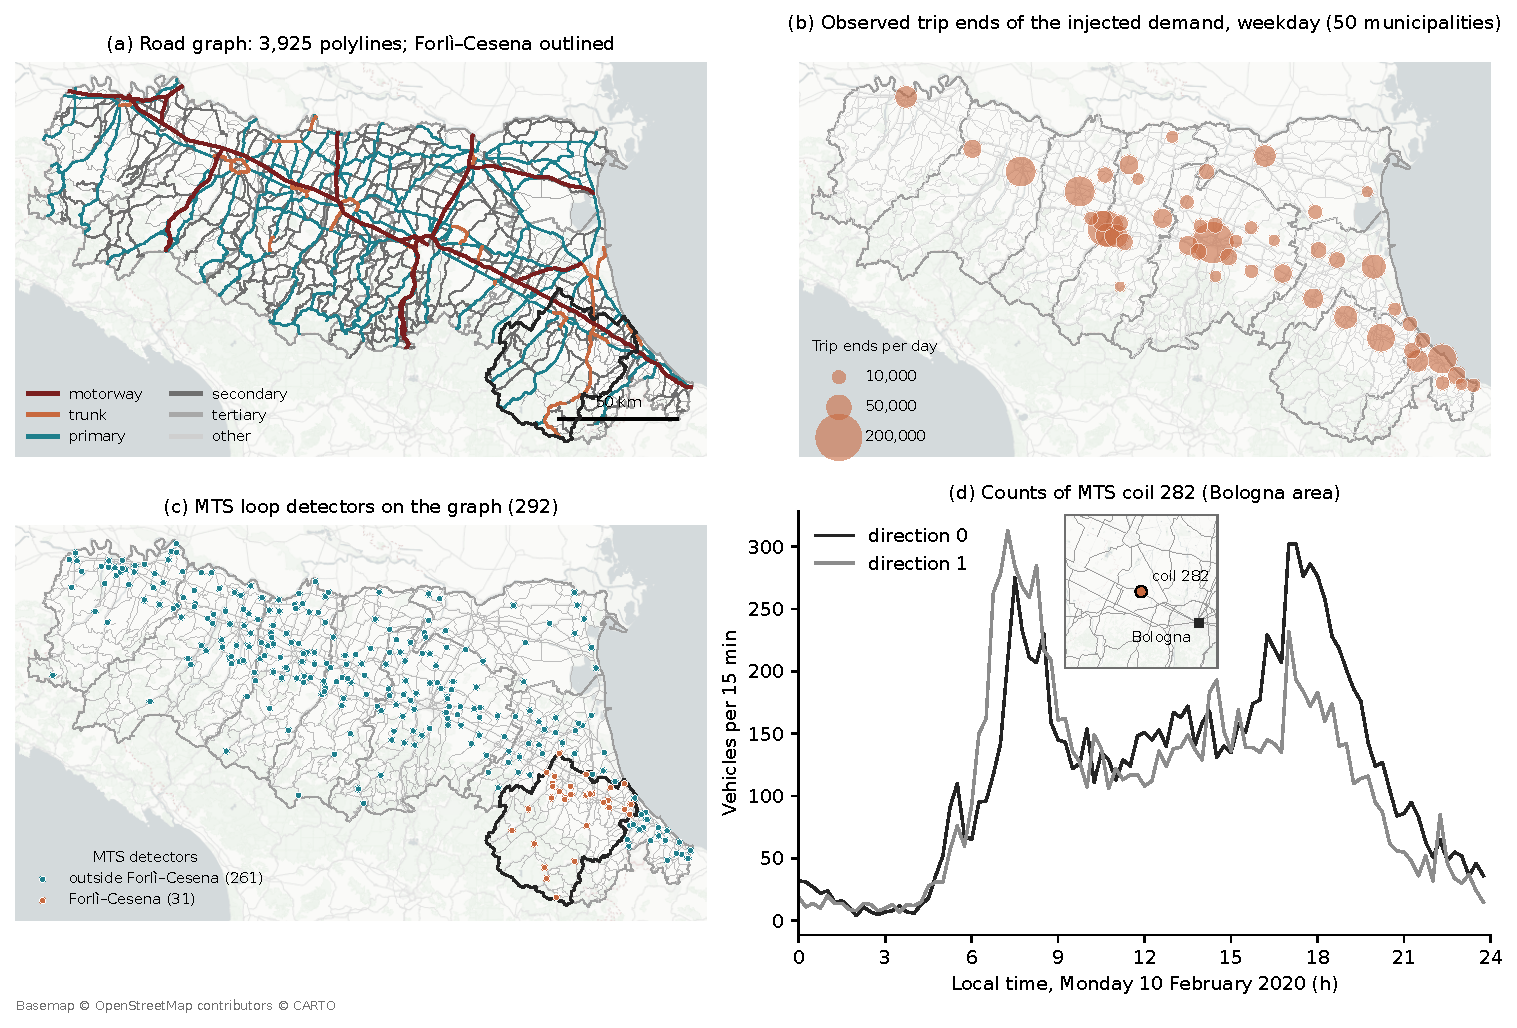
\includegraphics[width=\textwidth]{fig1_inputs.pdf}
\caption{\textbf{Regional domain and observational inputs.} \textbf{(a)} Model graph coloured by OpenStreetMap road class; the province of Forl\`i--Cesena, where GPS traces inform route choice, is outlined. \textbf{(b)} Daily trip ends with an observed endpoint in the weekday demand, by municipality. \textbf{(c)} MTS inductive loop detectors mapped to the graph. \textbf{(d)} Counts of coil 282 near Bologna on 10 February 2020, 15-min resolution, local time. Basemap \copyright{} OpenStreetMap contributors \copyright{} CARTO.}
\label{fig:inputs}
\end{figure*}

\begin{figure*}[htbp]
\centering
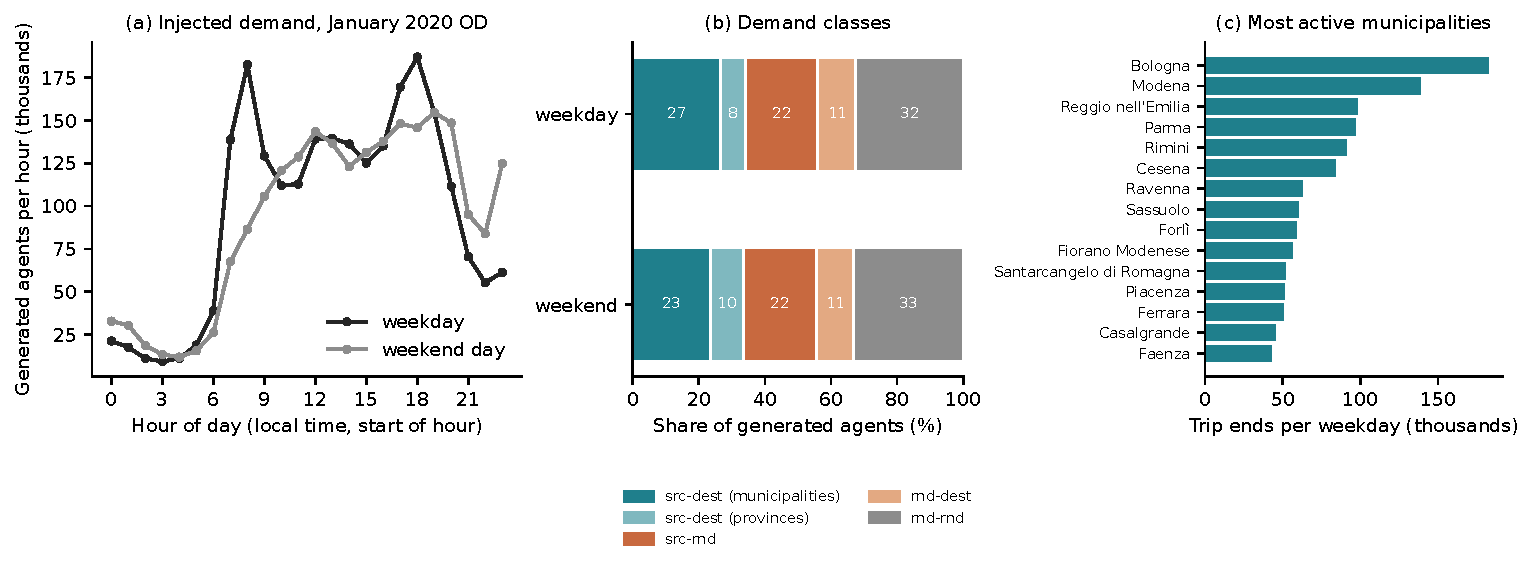
\includegraphics[width=\textwidth]{fig2_demand.pdf}
\caption{\textbf{Injected demand.} \textbf{(a)} Agents generated per hour for a weekday and a weekend day, after scaling by $k$. \textbf{(b)} Shares of the demand classes: observed origin and destination between municipalities or with provinces of neighbouring regions (src-dest), observed origin and random destination (src-rnd), random origin and observed destination (rnd-dest), and random origin and destination (rnd-rnd). \textbf{(c)} Municipalities with the most trip ends on a weekday.}
\label{fig:demand}
\end{figure*}

\subsection{Loop detectors}
The regional MTS system counts vehicles every 15~min in both directions; 292 detectors (called coils below) lie on links of the graph (Fig.~\ref{fig:inputs}c,d). Time stamps are in UTC and are converted to local time. For 2020 we use the project archive of the counts; for 2021 the regional open-data release of the same system (Regione Emilia-Romagna, CC BY), which in local time reproduces the archive for February 2020. A coil-day is used when both directions are complete for all 96 intervals.

\subsection{GPS probes}
Viasat provided hourly probe counts per matched link for two campaigns, 10--17 February 2020 (six weekdays and a weekend) and 28 June--4 July 2021 (five weekdays and a weekend), and the raw traces of private vehicles in the province of Forl\`i--Cesena. The matched links lie mainly in that province (Fig.~\ref{fig:viasat}). Probes did not enter demand generation, demand scaling or the detector correction.

\section{Methods}
\label{sec:methods}

\subsection{Agent-based simulation}
The \texttt{minimocas} agent-based model advances in 10~s steps. The speed of an agent is the speed of its link, reduced above a critical density. Source--destination agents follow best paths computed with a Dijkstra engine \cite{dijkstra1959} that respects turn restrictions; random-endpoint agents choose the next link at each node with probability proportional to a transition weight and travel within a time budget of 5,600~s. The simulator records, for each hour and direction, the number of distinct agents on each polyline, and virtual barriers at the coil locations count point crossings. Assignment is not equilibrated \cite{wardrop1952}, and the model does not resolve the congestion phenomena of microscopic traffic-flow models \cite{horni2016,lopez2018,treiber2013}. The simulator is deterministic.

\subsection{Route choice informed by GPS}
GPS fixes of private vehicles in Forl\`i--Cesena (February 2020) with engine on and speed of at least 5~km/h were matched to the nearest polyline within 20~m whose bearing agrees with the heading within 30$^\circ$. For each road class we take the median off-peak speed of the matched links (weekdays, 10:00--16:00) and the median daily number of probes per covered link (Table~\ref{tab:classes}); both are applied to all links of the class in the region. Speeds of the same roads in June 2021 have a rank correlation of 0.98 with those of February 2020. The probe numbers set the transition weights of random-endpoint agents and enter the best-path cost of link $i$,
\begin{equation}
w_i = L_i\left[\alpha + (1-\alpha)\,\frac{1/c_i - 1/c_{\max}}{1/c_{\min} - 1/c_{\max}}\right],
\label{eq:route_cost}
\end{equation}
where $L_i$ is its length, $c_i$ the usage weight of its class and $\alpha=0.5$. This variant was selected among shortest-distance, travel-time, mixed and usage-weighted alternatives by the rank correlation between simulated daily volumes and GPS counts on the links of Forl\`i--Cesena on 10 February 2020 (0.54, against 0.47 for shortest-distance routing; Supplementary Section~S3); detectors played no role in the selection. When the turn-restricted search finds no feasible path for this cost, the agent uses the shortest-distance path (\tbd{N} next-node decisions in the fifteen simulated days).

\begin{table}[htbp]
\centering
\caption{Road-class properties estimated from private-vehicle GPS traces in Forl\`i--Cesena, February 2020: median off-peak speed of links with at least 50 matched points (interquartile range in brackets) and median daily probes per covered link. Both are applied to all links of each class in the region.}
\label{tab:classes}
\begin{tabular}{@{}lrrrr@{}}
\toprule
Road class & Links (speed) & Speed (km/h) & Links (usage) & Probes per day \\
\midrule
Motorway & 44 & 123 [120--124] & 61 & 130 \\
Trunk & 75 & 83 [76--95] & 76 & 79 \\
Primary & 151 & 55 [46--64] & 160 & 109 \\
Secondary & 245 & 51 [46--60] & 248 & 36 \\
Tertiary & 193 & 53 [43--59] & 227 & 21 \\
Unclassified & 42 & 49 [36--54] & 57 & 14 \\
\bottomrule
\end{tabular}
\end{table}

\subsection{Demand scale from detector counts}
The OD tables describe the operator's sample of travellers, so the number of agents must be scaled to the traffic level. We multiply every creation rate by one factor $k$, the inverse of the effective coverage, and estimate it from detector counts. The complete coils of 10 February 2020 are split into a calibration and a test half, stratified by province (seed 20261028). The day is simulated with $k=1,1.5,1.6,\dots,2,3$, and $k^*$ is the value at which the pooled simulated volume on the calibration coils equals the observed one, interpolated linearly between simulated values. The test half, the other days of 2020 and the 2021 campaign play no role in the choice. A single factor preserves the relative structure of the demand; a factor per demand class, fitted on simulations of each class alone, was rejected because link volumes are not additive in the classes (Supplementary Section~S2).

\subsection{Local detector correction}
Let $u_i(h)$ be the simulated count on the directed link of coil $i$ in hour $h$, $b_i(h)$ the crossings of the virtual barrier at the coil, and $c_i(h)$ the observed count after direction mapping; coils on the same directed link are averaged. The increment at the coil link is
\begin{equation}
\delta_i(h)=\begin{cases} c_i(h)-u_i(h) & \text{if } u_i(h)\ge 1 \text{ and } b_i(h)\ge 1,\\ 0 & \text{otherwise,}\end{cases}
\label{eq:coil_residual}
\end{equation}
so that the corrected count $\widetilde u_i(h)=u_i(h)+\delta_i(h)$ equals the observation wherever the simulation has traffic at the coil. The increment is propagated downstream and upstream: each adjacent link receives the increment of its parent multiplied by its own simulated share of the flows leaving (downstream) or entering (upstream) the common node, $\delta_{(n_2,n)}=\delta_{(n_1,n_2)}\,u_{(n_2,n)}/\sum_m u_{(n_2,m)}$. Each branch carries its own increment and path length. Propagation does not enter other coil links, and stops when the increment falls below one vehicle, after three links along a path, at a forbidden turn or at a closed link; negative counts are set to zero.

\subsection{Validation}
\label{sec:validation_methods}
\emph{Hourly profiles.} For each GPS-matched polyline we compare the hourly shares $p_i(h)$ and $q_i(h)$ of the reconstructed and GPS counts summed over the campaign days, both directions together, through
\begin{equation}
\mathrm{MAE}_i=\frac{100}{24}\sum_{h=0}^{23}|p_i(h)-q_i(h)|,
\label{eq:profile_error}
\end{equation}
in percentage points (pp); links with zero simulated or GPS total are excluded, and only links whose geometry is identical in the graph used for map matching are kept. Three profiles applied to every link serve as baselines: the injected OD profile, the mean normalized profile of the coil directions complete on all days of the subset, and the uniform profile. The ratio between probes and simulated vehicles on link $i$,
\begin{equation}
\eta_i=\frac{\sum_{d,h}\psi_i(d,h)}{\sum_{d,h}\phi_i(d,h)},
\label{eq:penetration}
\end{equation}
with $\psi_i$ the probes and $\phi_i$ the simulated vehicles, describes the GPS sampling.

\emph{Volumes.} Daily volumes of both directions are compared at coils with complete data, averaging over complete days, by the ratio of pooled simulated to observed volume, the Spearman correlation, the median absolute $\log_{10}$ ratio and the share of coils within a factor of two. The route-choice comparison uses 5,000 paired bootstrap resamples of coils (seed 20261028).

\emph{Local correction.} In the leave-one-detector-out test all coils of a polyline are removed from the correction in turn, and their observations are compared with the corrected reconstruction on that polyline; the error is $\sum|\widetilde u(h)-c(h)|/\sum c(h)$ over hours, directions and days. The effect of the correction on GPS links is summarized by network distance from the nearest coil, the minimum number of polylines between a link and any coil link. The dependence on propagation depth uses a fixed random 20\% of the complete coils of each 2020 day as test set (seed 20261027).

\section{Results}
\label{sec:results}

\subsection{Demand scale}
\tbd{k scan results paragraph.}

\subsection{Reconstructed traffic field}
\tbd{coil 282 withheld, map; Fig 3.}

\begin{figure*}[htbp]
\centering
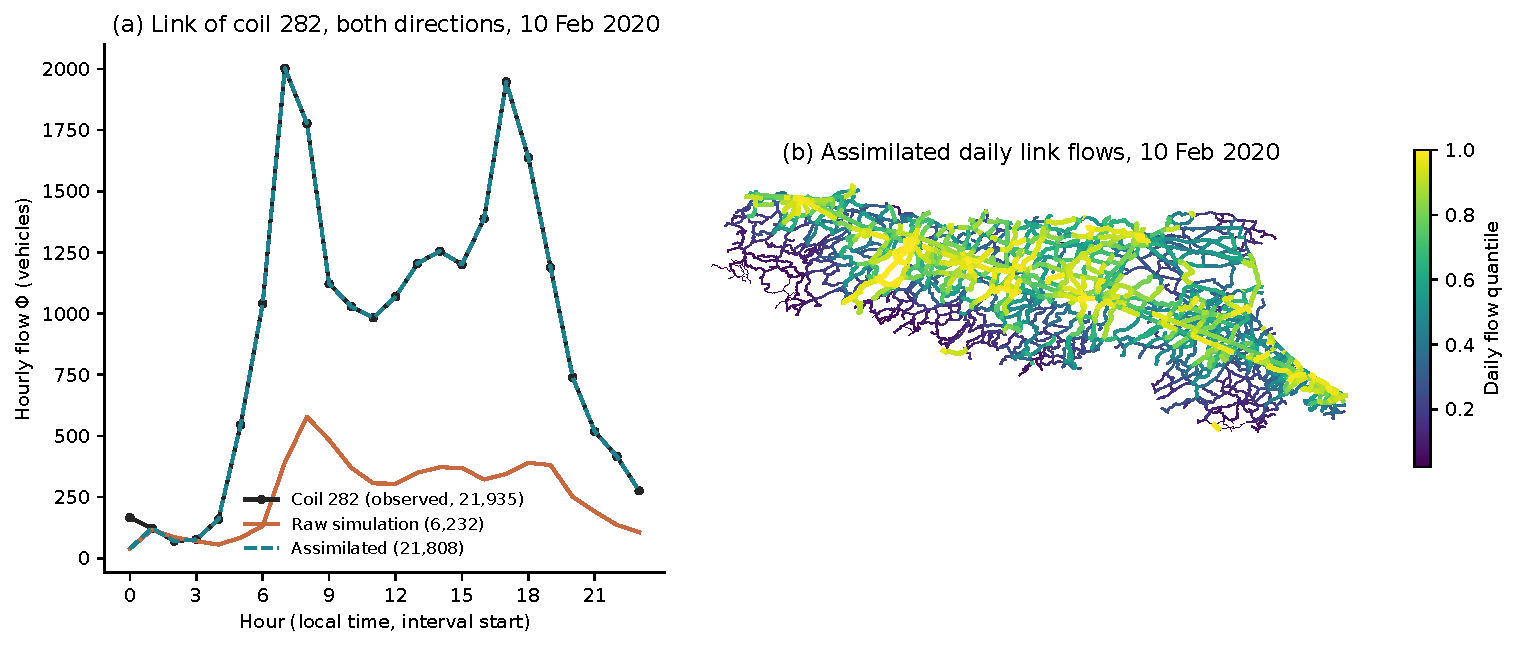
\includegraphics[width=\textwidth]{fig3_reconstruction.pdf}
\caption{\textbf{Reconstructed traffic field.} \textbf{(a)} Hourly counts of coil 282 (both directions) on 10 February 2020 and the reconstruction on its link when coil 282 is withheld from the correction and all other coils are assimilated; totals in parentheses. \textbf{(b)} Reconstructed daily link flows, coloured and scaled by flow quantile. Basemap \copyright{} OpenStreetMap contributors \copyright{} CARTO.}
\label{fig:simulation}
\end{figure*}

\subsection{Hourly profiles on all GPS-matched links}
\label{sec:all_links}
\tbd{profiles.}

\begin{figure*}[htbp]
\centering
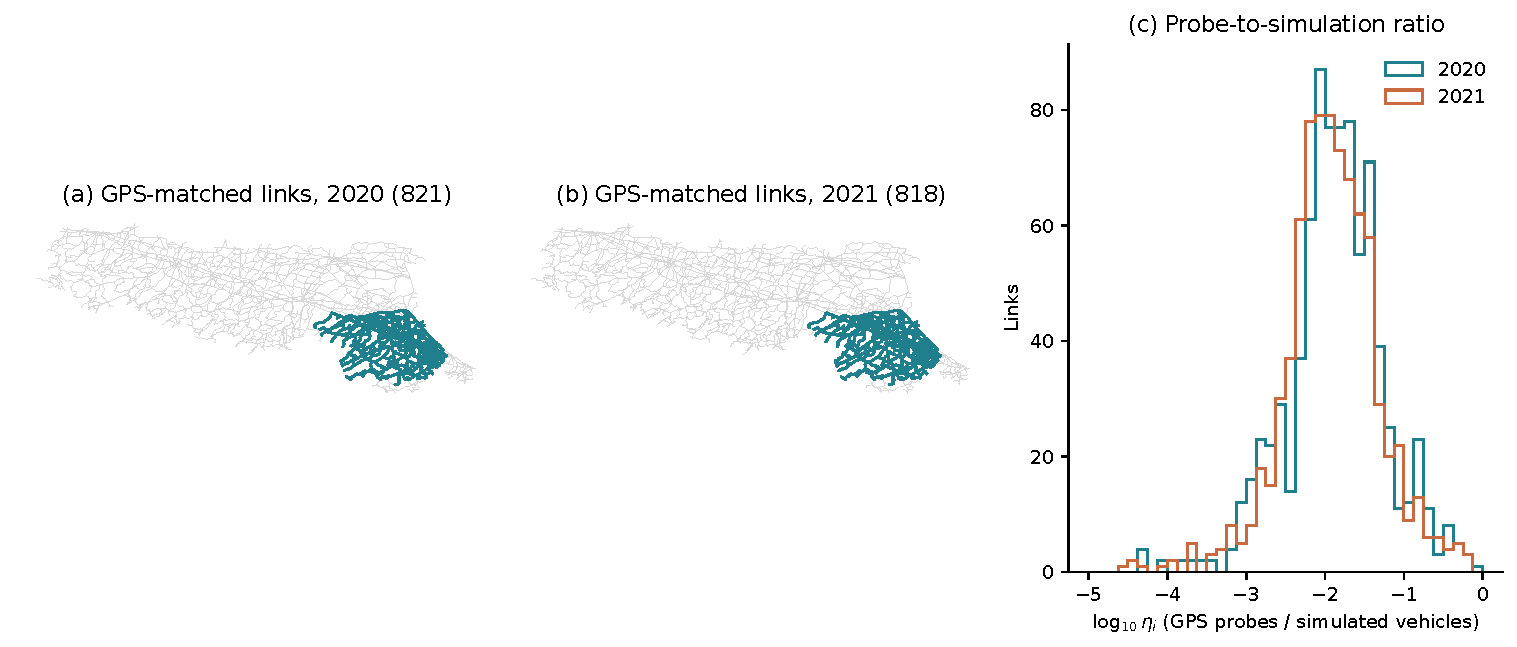
\includegraphics[width=\textwidth]{fig4_gps.pdf}
\caption{\textbf{GPS coverage.} \textbf{(a,b)} Usable GPS-matched links (number in parentheses) over the regional graph, 10--17 February 2020 and 28 June--4 July 2021. \textbf{(c)} Distribution of the link ratio $\eta_i$ between probe counts and simulated vehicles, Eq.~\eqref{eq:penetration}. Basemap \copyright{} OpenStreetMap contributors \copyright{} CARTO.}
\label{fig:viasat}
\end{figure*}

\begin{figure*}[htbp]
\centering
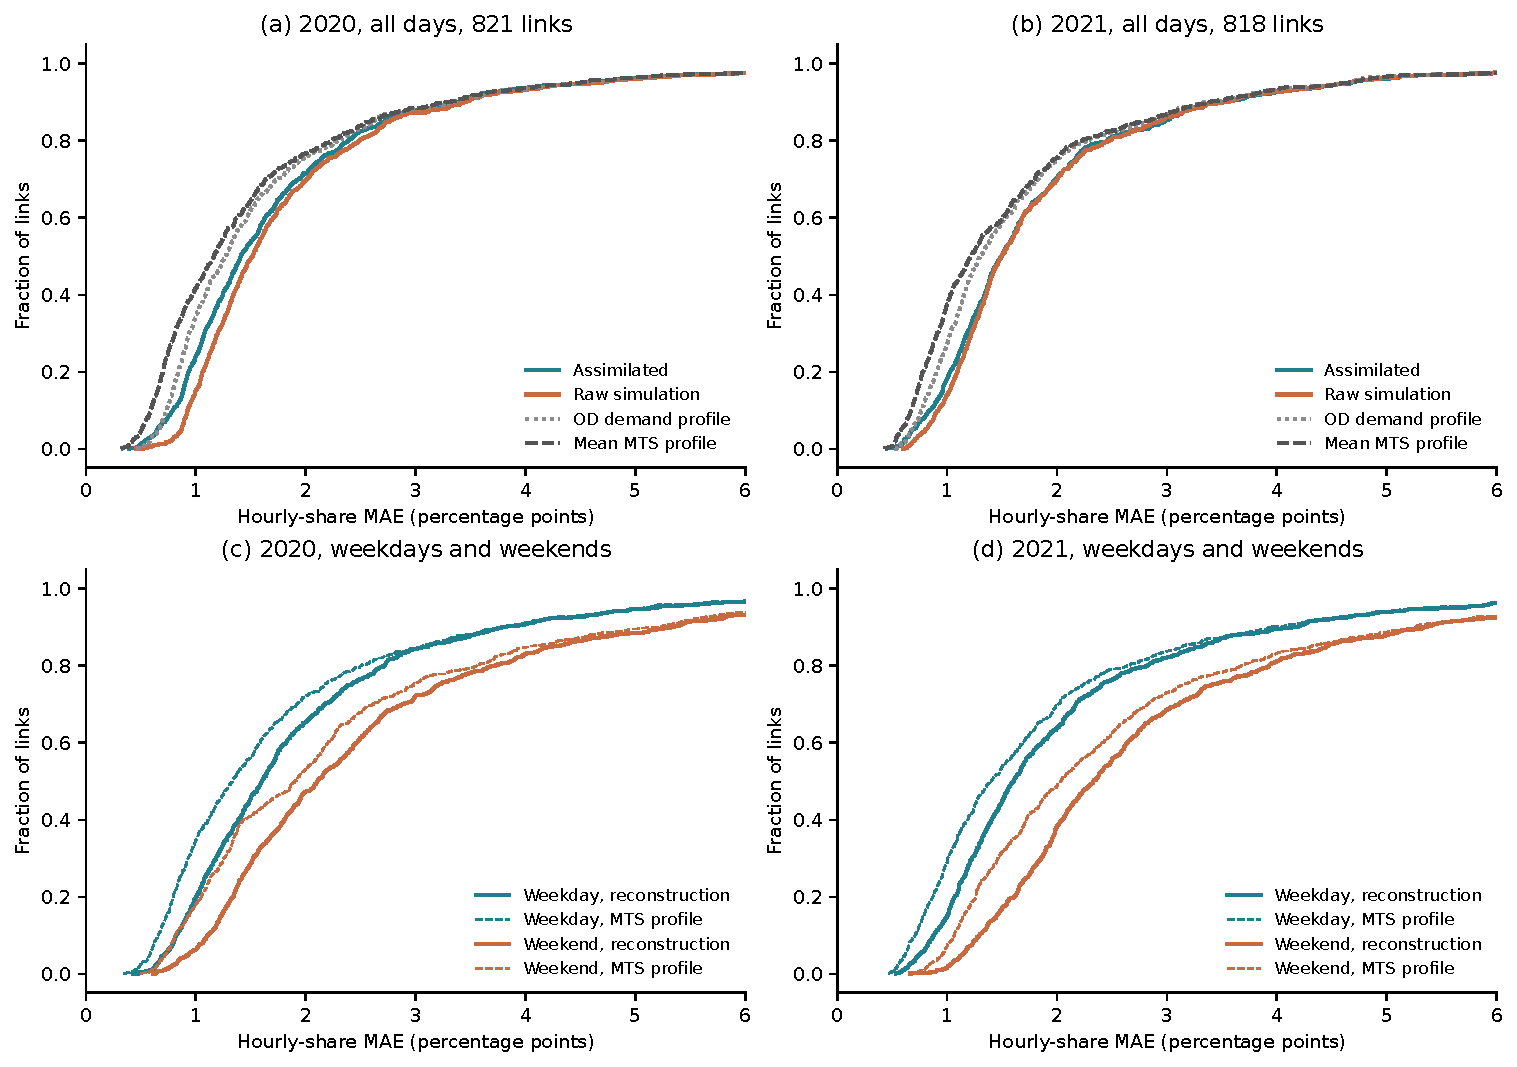
\includegraphics[width=\textwidth]{fig5_validation.pdf}
\caption{\textbf{Hourly-share validation on all usable matched links.} \textbf{(a,b)} Cumulative distributions of the link MAE for the reconstruction, the OD demand profile and the mean MTS profile. \textbf{(c,d)} Reconstruction and MTS profile on weekdays and weekends; curves extend beyond the 6~pp limit.}
\label{fig:validation_cdf}
\end{figure*}

\subsection{Volumes at independent detectors}
\tbd{volumes.}

\subsection{Reach of the local correction}
\tbd{reach.}

\begin{figure*}[htbp]
\centering
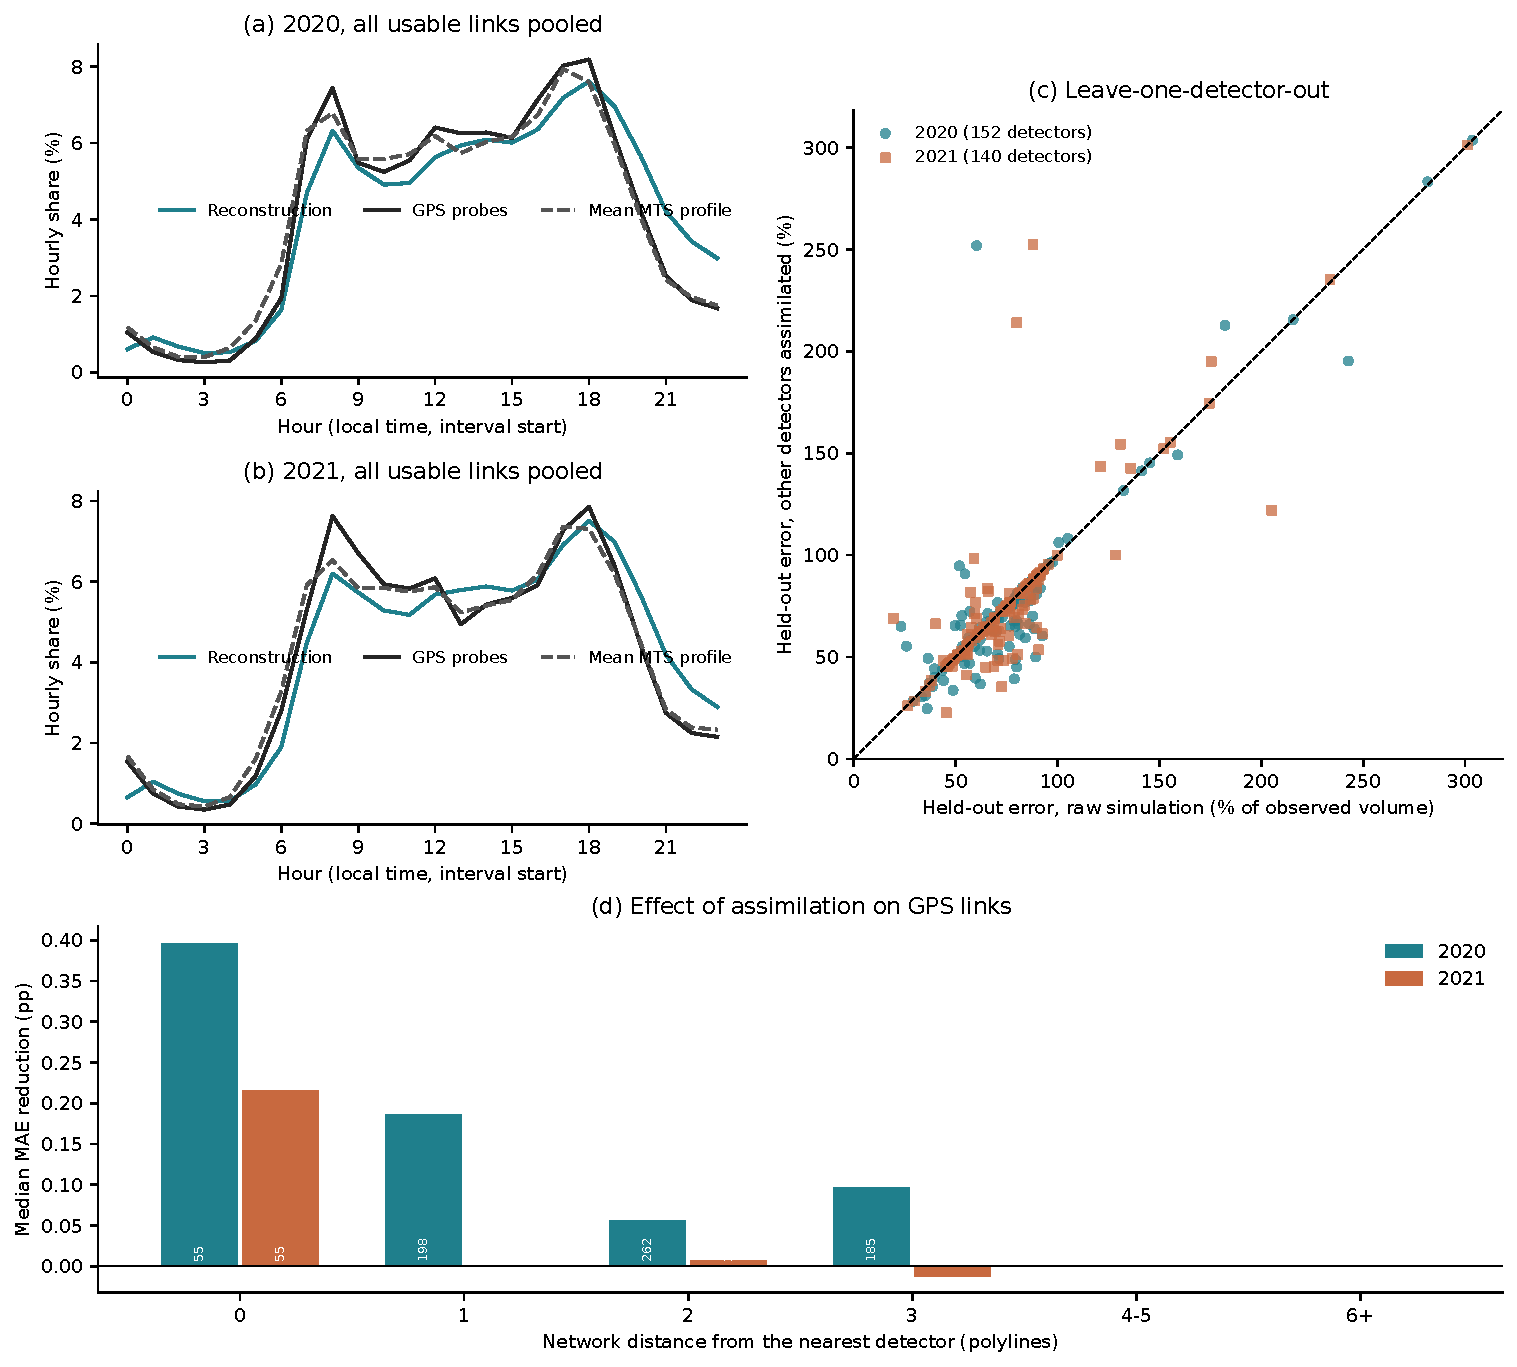
\includegraphics[width=\textwidth]{fig6_diagnostics.pdf}
\caption{\textbf{Timing and reach of the correction.} \textbf{(a,b)} Hourly shares pooled over all usable links: reconstruction, GPS probes and mean MTS profile. Pooling weights links by their own volumes, so these curves are not regional traffic shares. \textbf{(c)} Median reduction of the hourly-share error on GPS links by network distance from the nearest coil, in polylines, for 2020 and 2021.}
\label{fig:diagnostics}
\end{figure*}

\begin{figure*}[htbp]
\centering
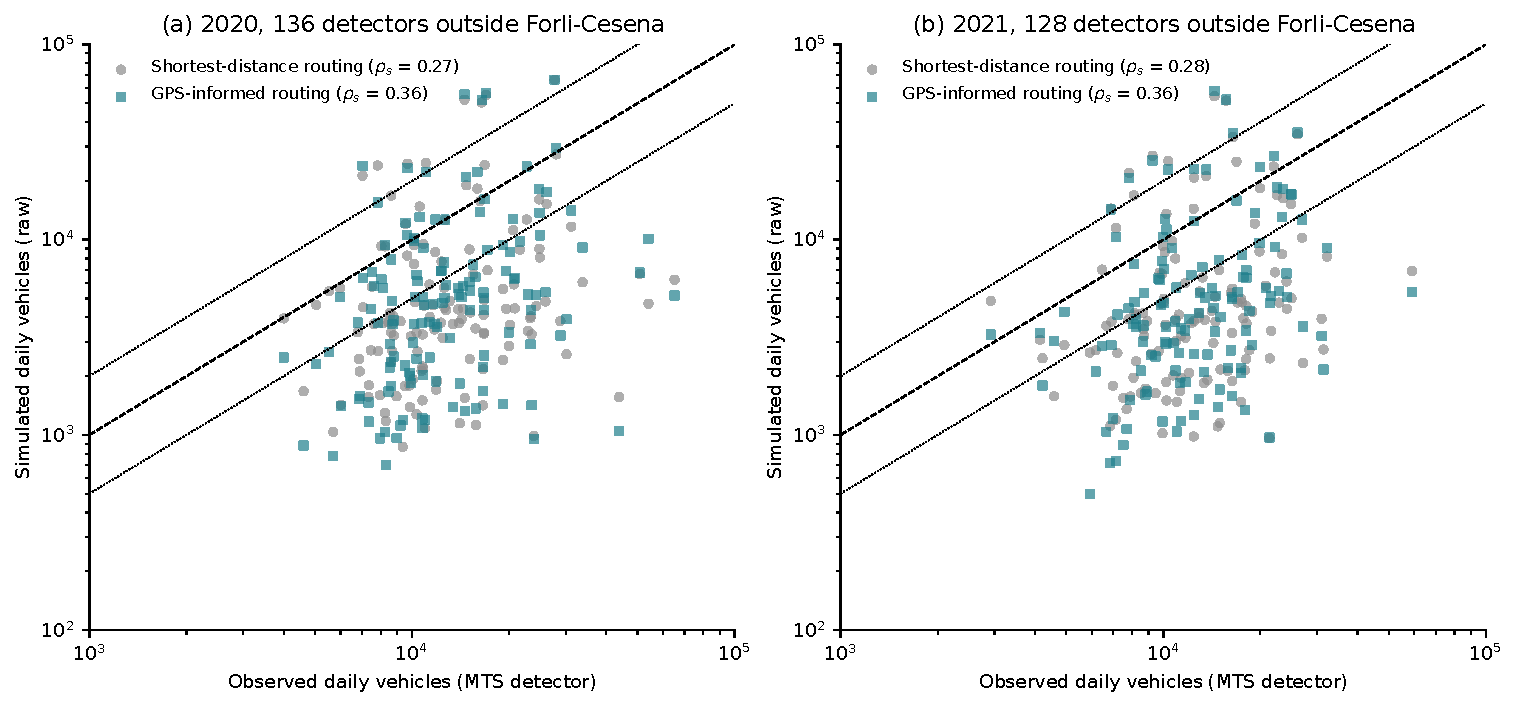
\includegraphics[width=\textwidth]{fig7_volumes.pdf}
\caption{\textbf{Daily volumes at withheld detectors.} Observed daily volume of each coil (mean over complete days, both directions) against the reconstruction on its link when the coil is withheld from the correction and all other coils are assimilated, \textbf{(a)} 10--17 February 2020 and \textbf{(b)} 28 June--4 July 2021. Coils reached by the correction propagated from other coils are distinguished from those that are not; $\rho_s$, Spearman correlation. Dashed line: equality; dotted lines: factor of two.}
\label{fig:loo_volumes}
\end{figure*}

\section{Discussion}
\label{sec:discussion}
\tbd{discussion.}

\section{Conclusions}
\label{sec:conclusions}
\tbd{conclusions.}

\section*{Abbreviations}
GPS, Global Positioning System; MAE, mean absolute error; MTS, regional traffic monitoring system of Emilia-Romagna; OD, origin--destination; pp, percentage points.

\section*{Supplementary Information}

The Supplementary Material describes the data layers and the demand classes (S1), the demand scale and the rejected per-class alternative (S2), the route-choice variants (S3), the detector correction and its sensitivity to propagation depth (S4), additional validation results (S5) and the reproduction of all results (S6).

\section*{Availability of data and materials}

The mobile-phone OD tables (TIM) and the Viasat GPS data are proprietary and were used under agreements that do not allow redistribution; requests for access should be addressed to the data providers. MTS loop-detector counts are published by Regione Emilia-Romagna under a CC BY licence (open-data catalogue, dataset ``Sistema MTS -- Flussi di traffico al quarto d'ora''). Road classes are derived from OpenStreetMap (\copyright{} OpenStreetMap contributors, ODbL). The road graph, the simulation configurations, the aggregate results behind every figure and table, and the link-level validation metrics without probe counts are included in the code repository.

\section*{Code availability}

The simulator \texttt{minimocas}, the detector correction and all analysis scripts are available at \url{https://github.com/federicobellisardi/multi-sensor-traffic-reconstruction} (directory \texttt{article1/analysis}); Supplementary Section~S6 lists the commands that reproduce each result.

\section*{Ethics approval and consent to participate}

Mobile-phone data were provided by the operator as anonymized OD counts aggregated in space and time; no individual-level records were accessed. GPS data were provided as pseudonymized vehicle records and were used only to compute link counts, speeds and road-class aggregates. No personal data are reported, and ethics approval was not required.

\section*{Competing interests}

C.M. and A.F. are employed by Mindicity, which contributed to the development of the modelling framework. The other authors declare no competing interests.

\section*{Funding}

F.B. received support from the Italian National Operational Programme on Research and Innovation 2014--2020 (CCI 2014IT16M2OP005), FSE REACT-EU, Actions IV.4 and IV.5.

\section*{Authors' contributions}

F.B. designed the study, developed the reconstruction and validation pipeline, performed the analyses and wrote the manuscript. C.M. and A.F. contributed to the simulation framework and to the processing of the mobile-phone and detector data. A.B. conceived the modelling approach and supervised the study. All authors read and approved the final manuscript.

\section*{Acknowledgements}

We thank TIM (Telecom Italia) for the mobile-phone data, Viasat for the GPS data, the Mobility and Viability Section of the Emilia-Romagna Region for the MTS detector data, and Stefano Grandi, Claudio Domenichini and Elena Grossi for discussions.

\bibliographystyle{unsrtnat}
\bibliography{references}
\end{document}


